\documentclass{article}

\usepackage[utf8]{inputenc}
\usepackage[ngerman]{babel} 
\usepackage{fancyhdr}
\usepackage{tabularx}
\usepackage{graphicx}
\usepackage{lastpage}
\usepackage{ltablex}
\usepackage{lipsum}
%\usepackage{lscape} % ohne Ändern der Seite
\usepackage{pdflscape} % mit Ändern der Seite
\usepackage{colortbl}

\definecolor{red}{RGB}{255,0,0}
\definecolor{orange}{RGB}{255,165,0}
\definecolor{yellow}{RGB}{255,255,0}
\definecolor{green}{RGB}{0,255,0}


\newcolumntype{L}[1]{>{\raggedright\arraybackslash}p{#1}}
\newcolumntype{C}[1]{>{\centering\arraybackslash}p{#1}}
\newcolumntype{R}[1]{>{\raggedleft\arraybackslash}p{#1}}

\usepackage[
%showframe,% Seitenlayout anzeigen
left=3cm,
right=2cm,
top=2.5cm,
bottom=2cm,
%includeheadfoot
]{geometry}

\pagenumbering{arabic}


\begin{document}
\title{%
	Fallstudie Home-Computer \\
	\large Information Security Fundamentals \\
	Hochschule Luzern}

\author{Florian Bär}
\maketitle
\thispagestyle{empty}
\clearpage
\setcounter{page}{1}

\tableofcontents

\section{Einführung zum Minicase}

Die Familie Meier wohnt in einem dreistöckigen Haus im zweiten Stockwerk. Insgesamt teilen 6 Wohnungen das Haus auf. Eine fortschrittliche Familie aus dem Mittelstand mit bester Reputation.
Bei der Familie Meier wird die IT-Infrastruktur von Onkel Smirnow betreut, welcher von Zeit zu Zeit mit Cracks und anderen Tools das Leben der Familie Meier vereinfacht.


Es folgt der Netzwerkaufbau der Familie Meier zur Veranschaulichung.


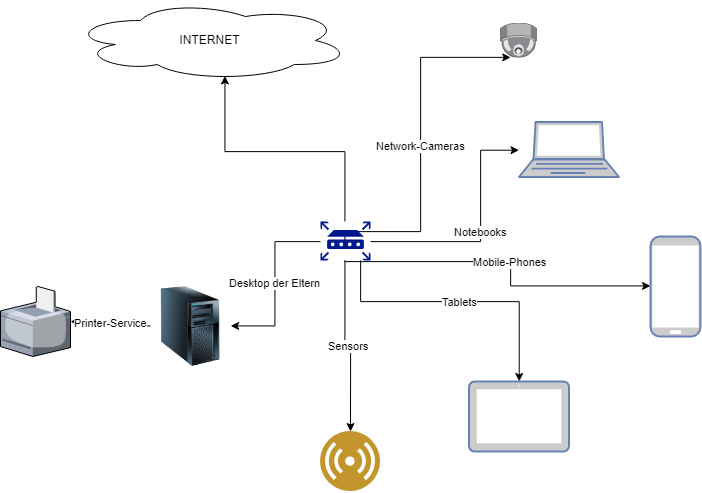
\includegraphics[width=14cm]{./Netzwerk.png}

Für diese Familie sollte ein Massnahmenplan für allfällige Risiken gemäss der Aufgabenstellung \grqq Fallstudie: Die Heim PC Lösung\grqq \space erstellt werden. Für die Eintrittswahrscheinlichkeit und den potenziellen Schaden (Schadensausmass) der Ereignisse wird eine Skala von 1 (sehr kleine(r) Wahrscheinlichkeit/Schaden) bis 4 (sehr grosse(r) Wahrscheinlichkeit/Schaden) verwendet.



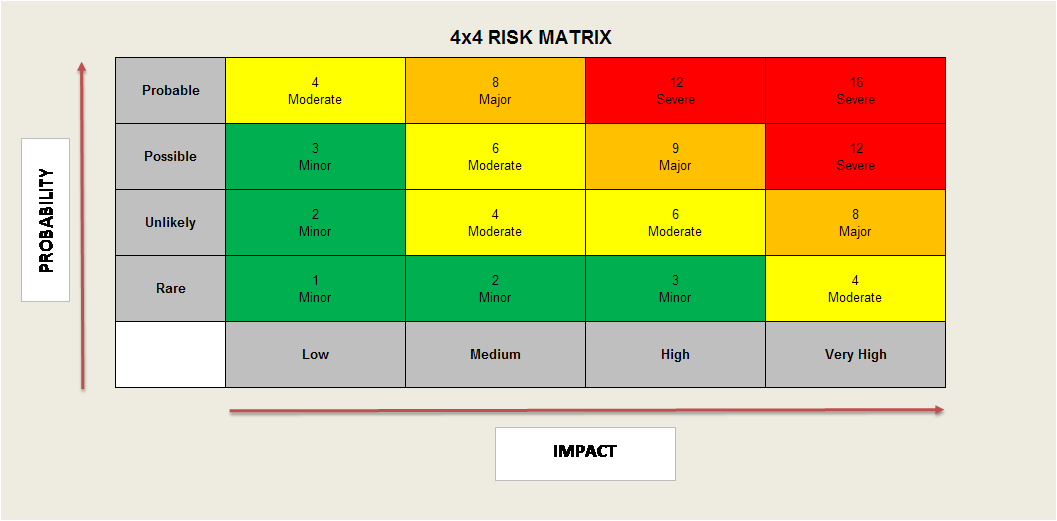
\includegraphics[width=\textwidth]{./Risikomatrix.png}


\newpage


\section{Fallstudie ISF}

\subsection{Risiken}

\subsubsection{Beschreibung der Risiken}

Es folgt eine Liste mit Dingen, welche Sicherheitsrisiken beinhalten:
\begin{enumerate}
\item Das Wireless brauch WEP. WEP ist veraltet und nicht sicher. Es ist ein upgrade
zu WPA2 empfohlen.
\item Die Spiele und Tools, welche Onkel Özutück mitbringt, könnten gecrackt sein.
Cracks beinhalten ein Sicherheitsrisiko. Selbst wenn Sie nicht gefährlich sind, dann
sind diese illegal verwendet.
\item Da Jan ein Computerfreak ist, versucht er bestimmt immer neue Dinge. Dabei wird das Sicherheitsrisiko von diesen “Nerd”-Tools oftmals unterschätzt.
\item Dora ist mit 12 Jahren ein junges Kind. Vor allem bei jungen Kindern sollte der
Internetkonsum kontrolliert werden. Dazu gibt es passende Kinderschutzsoftware.
\item Die Computer müssten auf einem NAS oder einem sonstigen Server ein Backup
haben. Falls einmal eine HD kaputt gehen sollte, sind die Daten nicht wiederherstellbar.
\item Die Kameras könnten von einem Billighersteller sein, welcher die Sicherheitsysteme
des Systems nicht sehr verantwortungsvoll implementiert. Diese könnten dann
“gehackt” werden und einen grossen Eingriff in die Privatsphäre der Familie.
\item Der Desktop PC der Eltern sollte nicht gleichzeitig als PC und als Printserver
verwendet werden. Server öffnen normalerweise Ports und Services für das Netzwerk
und können so ein Sicherheitsrisiko darstellen.
\item Windows Betriebssysteme besitzen zwar den Bitlocker, jedoch ist dieser Standard-
mässig nicht eingeschaltet und kann auch nur von forgeschrittenen Usern bedient
werden. Dadurch sind die Daten auf den Disks nicht verschlüsselt und können unter
Umständen ausgelesen werden.
\item Bei einem Brand wären alle Computer zerstört und es könnten keine Daten wieder-
hergestellt werden.
\item Benutzen die Kinder und die Eltern die selbe Mail? Dies könnte allenfalls auch zu
einem Risiko werden. Nicht alle Mails sind für die Augen der Kinder gedacht.
\end{enumerate}
\newpage

\begin{landscape}

\subsubsection{Risikomatrix}
\begin{tabularx}{\columnwidth}{|r|c|X|c|X|c|}
	\hline
	\textbf{ID} & \textbf{EW\footnote{Eintrittswahrscheinlichkeit}} & \textbf{Begründung} & \textbf{SG\footnote{Schadensgrösse}} & \textbf{Begründung} & \textbf{Risiko} \\ 
	\hline		
	1 &  \cellcolor{red}4 & Da WEP schon veraltet ist und in wenigen Sekunden mit einem mittelklassigen Computer geknackt werden kann ist die Eintrittswahrscheinlichkeit hoch. & \cellcolor{red}4 & Mit Zugriff auf das Netzwerk ist dem “Hacker” alles Möglich	(Zugriff auf Computer, Kameras etc.).  & \cellcolor{red}16 \\ \hline
	2 &  \cellcolor{red}4 & Sehr hoch, da im Text steht, dass der Onkel Özukück gratis Software mitbringt.  & \cellcolor{red}4 & Da Cracks häufig infiziert sind, ist das Risiko für das infizieren mit einer Schadsoftware sehr gross.  & \cellcolor{red}16 \\ \hline
	3 &  \cellcolor{orange}3 &  Es gibt auch auf Github und anderen Clouddiensten viele Schadsoftware, welche als kleine Tools getarnt sind.  & \cellcolor{red}4 & Wenn der PC mit Schadsoftware infiziert wurde, dann ist dieser Computer dieser ausgeliefert.  & \cellcolor{red}12 \\ \hline
	4 &  \cellcolor{red}4 & Da Kinder tendenziell sich am PC explorativ verhalten, kann Dora einfach auf zwilichtige Webseiten gelangen.  & \cellcolor{red}4 & Der Besuch von "schlechten" Webseiten kann die Zukunft von Dora massiv beeinflussen und im schlimmsten Fall dazu führen, dass sie einmal im Gefängnis landet. & \cellcolor{red}16 \\ \hline
	5 &  \cellcolor{orange}3 & Es kann immer einmal ein Laptop auf den Boden fallen. Falls dann eine HD kaputt geht, sind allenfalls gespeicherte Fotos auf diesem Computer verloren. Auch von einer allfälligen Fehlproduktion ist man nicht geschützt. & \cellcolor{orange}3 & Der materielle Schaden ist bei der Familie nicht sehr gross. Allerdings kann der Verlust von Familienfotos sehr schmerzhaft sein. & \cellcolor{orange}9 \\ \hline
	6 &  \cellcolor{yellow}2 & Auch Billigkamerahersteller bemüht, das Sicherheit einem Minimalstandard entspricht. & \cellcolor{orange}3 & Das Interesse von einem Hacker, sich Zugriff auf eine Kamera zu verschaffen ist allerhöchstens von perversem Interesse. & \cellcolor{yellow}6 \\ \hline\textsl{}
	7 &  \cellcolor{yellow}2 & Games und Server öffnen Services für die Multiplayerfähigkeit. Diese stellen potenziell ein Sicherheitsrisiko dar. & \cellcolor{red}4 & Wenn man mit einem Bufferoverflow oder anderen Code-Injection sich Zugriff auf einen PC erschleichen kann, dann ist man Herr über dieses Gerät. & \cellcolor{orange}8 \\ \hline
	8 &  \cellcolor{yellow}2 & Damit man an die Daten des Computers kommt, muss man zuerst Zugriff auf diesen Computer haben. Dies ist nur bei einem Einbruch oder einem Diebstahl möglich. & \cellcolor{orange}3 & Wenn man allerdings einmal Zugriff auf diesen Computer hat, dann ist es einer Fremdperson möglich, alle Daten\footnote{inkl. Passwörter und persönliche Unterlagen} auszulesen.  & \cellcolor{yellow}6 \\ \hline
	9 &  \cellcolor{yellow}2 & Dass alle Daten und Backups zerstört werden ist grundsätzlich nur bei einem Brand möglich. Diese sind in der Schweiz zum Glück selten. & \cellcolor{red}4 & Wenn ein Brand ausbrechen würde, dann wären alle Daten und auch deren (allenfalls gemachten) Back-Ups zerstört. & \cellcolor{orange}8 \\ \hline
	10 &  \cellcolor{orange}3 & Normalerweise interessieren sich die Kinder nicht für die Mails der Eltern. Und um Schaden zu verursachen, müsste dies Mutwillig seitens der Kinder geschehen. & \cellcolor{yellow}2 & Die Eltern haben normalerweise nicht viele (bis keine) Information, welche Schaden anrichten können. & \cellcolor{yellow}6 \\ \hline
\end{tabularx}

\newpage

\end{landscape}



\include{Risikomatrix}



\subsection{Massnahmen}

\subsubsection{Beschreibung der Massnahmen}
\begin{enumerate}

\item WEP mit WPA2 ersetzen und somit das Netzwerk von fremden Zugriff schützen. Zudem mit einem neueren Router mit Guest-Zugriff die Netzwerke trennen.

\item Software von einem vertrauenswürdigen Anbieter kaufen anstatt vom Onkel gecrackt mitbringen lassen.

\item Alle Netzwerkgeräte mit einem Anti-Virus ausstatten um allfällige Infektionen frühzeitig erkennen.

\item Dora nur ein Laptop mit “Kindersicherung” geben. Dazu Dora keine Administra-
torenrechte geben. Diese Rechte reichen dem Kind. Falls Dora weiter Software benötigt, muss Sie diese bei den Eltern erhalten.

\item NAS kaufen, um ein Backup von Daten zu machen. Auf dem NAS ein RAID 6 konfigurieren, damit auch auf dem NAS allfällige Dateiverluste vermieden werden können.

\item Einen zweiten Router kaufen, um die Sensoren und Kameras in ein anderes Netz
zu stellen.
• Durch diese Netztrennung, ist das Heimnetz von allfälligen Hackerangriffen
besser geschützt.



\item Ein Netzwerkdrucker kaufen, welcher von allen Netzwerkgeräten ein Drucken zulässt. Das in Massnahme 5 NAS könnte auch mittels Docker einen PrinterServer hosten, was auch das Problem der geöffneten Ports des Arbeits-PCs löst.


\item Windows 10 Pro kaufen und damit Bitlocker einschalten, welcher die Disk verschlüsselt. Alternativ kann auch eine Linux-Distribution verwendet werden, welche dieses Feature bereits gratis anbietet.

\item Mit einer Online-Backup-Lösung (Acronis Cloud / Google Cloud / Backblaze etc...) kann einfach und kostengünstig Cloud-Storage verwendet werden. Somit sind die Daten Ortsunabhängig gespeichert und auch bei einem Brand sind keine Daten verloren sondern wiederherstellbar


\item Für jede Person im Haushalt ein eigenes Windows Konto und ein eigenes Mail-Konto erstellen. Somit ist der gegenseitige Zugriff verwährt. 




\end{enumerate}

\begin{landscape}
	\newpage
	\subsubsection{Risikomatrix nach Massnahmen}
	
	\begin{tabularx}{\columnwidth}{|r|c|X|c|X|c|c|}
		\hline
		\textbf{ID} & \textbf{EW\footnote{Eintrittswahrscheinlichkeit}} & \textbf{Begründung} & \textbf{SG\footnote{Schadensgrösse}} & \textbf{Begründung} & \textbf{neues Risiko} & \textbf{Anwendbar\footnote{Massnahme einfach anwendbar}} \\ 
		\hline
		1 &  \cellcolor{green}1 & Auf dem Router anstelle von WEP ein WPA2 Passwort setzen. WPA2 ist viel schwerer zu intercepten und somit besteht ein geringers Risiko von einem unerwünschten Zugriff. & \cellcolor{yellow}2 & Falls einer Fremden Person der Zugriff auf das Netzwerk trotzdem gelingen sollte, ist man nicht vor Schaden geschützt. & \cellcolor{green}2 & \cellcolor{green} Ja  \\ \hline
		
		2 &  \cellcolor{green}1 & Spiele können trotzdem ungewollt Ports eines Systemes öffnen und damit ein Risiko darstellen. Zudem könne Mods Sicherheitslücken beinhalten und ein Problem darstellen. Das Risiko, welches Crack mitbringen ist allerdings eliminiert. & \cellcolor{yellow}2 & Das Risiko, welches von gekaufter Software ausgeht ist mit Massnahme (3) gelöst & \cellcolor{green}2 & \cellcolor{green} Ja  \\ \hline
		
		3 &  \cellcolor{yellow}2 & Mods und kleinere Informatik-Tools welche Schadcode enthalten können, werden von einem Virenscanner frühzeitig erkannt und eliminiert. & \cellcolor{green}1 & Falls doch eine Schadsoftware aufgrund der Dateisignatur unerkannt bleiben sollte, dann erkennt ein Antivirus aufgrund von Verhaltensmustern die Schadsoftware und der Schaden bleibt gering. & \cellcolor{green}2 & \cellcolor{green} Ja \\ \hline

		4 &  \cellcolor{green}1 & Dora kann nun keine unerwünschte Software mehr installieren und von Ihr geht somit keine Gefahr mehr aus. & \cellcolor{yellow}2 & Dora kann die Computer im eigenen Netzwerk nicht mer infizieren und somit keinen Schaden verursachen.  & \cellcolor{green}2 & \cellcolor{green} Ja  \\ \hline
		
		5 &  \cellcolor{yellow}2 & Es ist immernoch Möglich, dass eine Disk oder ein Computer kaputt geht. Auch wenn eine Disk auf dem NAS kaputt geht, besteht kein Schaden, da das auf dem NAS ein RAID 6 konfiguriert ist. & \cellcolor{green}1 & Falls eine Harddisk kaputt geht, sind Backups der jeweiligen Systeme vorhanden welche zurückgespielt werden können. & \cellcolor{green}1 & \cellcolor{green} Ja  \\ \hline
		
		6 &  \cellcolor{yellow}2 & Falls die Kameras und Sensoren unsicher sind, können diese immernoch geknackt werden. & \cellcolor{yellow}2 & Es besteht kein Netzwerkzugriff mehr, falls diese Geräte gehackt werden. Allerdings hat der potenzielle Eindringling danach zugriff auf die Kameras und kann die Familie beobachten. Dieses Risiko besteht allerdings immer, wenn man Netzwerkkameras hat. & \cellcolor{yellow}4 & \cellcolor{green} Ja  \\ \hline
		
		7 &  \cellcolor{green}1 & Der Fremdzugriff auf den PC aufgrund des Printservices ist nicht mehr Möglich. & \cellcolor{green}1 & Wenn es einem Hacker möglich ist, auf den Drucker zuzugreiffen, dann kann dieser nur noch Dokumente ausdrucken. & \cellcolor{green}1 & \cellcolor{green} Ja  \\ \hline
		
		8 &  \cellcolor{yellow}2 & Wenn die HardDisk verschlüsselt ist, dann sind die Daten der Familie geschützt und es kann nur noch die Hardware verwendet werden\footnote{dies ist zwar Schade, allerdings kein Sicherheitsrisiko}. & \cellcolor{green}1 & Der Zugriff auf die Computer bei einem Diebstahl ist erschwert und die Daten auf diesen Computern sind besser geschützt. Der Zugriff auf die Daten der Familie ist geschützt. & \cellcolor{green}2 & \cellcolor{green} Ja  \\ \hline
		
		9 &  \cellcolor{yellow}2 &  Ein Brand kann immernoch ausbrechen, ist in der Schweiz allerdings immernoch selten. & \cellcolor{green}1 & Daten sind nun Zentral gesichert. Bei einem allfälligen Hardware-Defekt des NAS oder einem Brand sind die Daten auf dem Netzwerkspeicher nicht verloren. & \cellcolor{green}2 & \cellcolor{green} Ja  \\ \hline
		
		10 &  \cellcolor{green}1 & Wenn jede Person im Haushalt ein eigenes Konto hat, dann ist der gegenseitige Zugriff verwährt. & \cellcolor{yellow}2 & Wenn ein Familienmitglied jedoch etwas "dummes" mit dem eigenen Konto macht, dann muss diese auch die Verantwortung übernehmen und ist klar idientifizierbar. & \cellcolor{green}2 & \cellcolor{green} Ja  \\ \hline
		
	\end{tabularx}
	
	
\end{landscape}

\section{Fazit}

Die Familie Meier hatte gemäss der Beschreibung der Fallstudie grosse Sicherheitsdefizite. Gründe für diese bestehenden Risiken sind auf die folgenden Punkte zurückzuführen:
\begin{itemize}
	\item Naivität
	\item Faulheit
	\item Unwissen
\end{itemize}
Die Familie Meier kann bereits mit geringem Aufwand grosse Risiken eliminieren. Diese Massnahmen benötigen jedoch einen Geldbetrag von bis zu CHF 5000.- aufgrund der Kosten für ein NAS und allfällige Cloud-Services welche gemietet werden müssen. Hinzu kommen die Kosten für die Software, welche nun gekauft werden müssen (da die Familie Meier den Kontakt zu Onkel Özutück abgebrochen hat).

Mit den in disesem Dokument enthaltenen Massnahmen konnte die Gesamt-Risko Summe von 103 Risikopunkten auf 20 Risikopunkte minimiert werden. Dies entspricht einer Reduktion von 515\%. 

\end{document}
